\documentclass[11pt]{article}

\usepackage[margin=1in]{geometry}
\usepackage{graphicx}
\usepackage{booktabs}
\usepackage{xcolor}
\usepackage{microtype}
\usepackage{caption}
\usepackage{subcaption}
\usepackage{enumitem}
\usepackage{titlesec}
\usepackage{pgfplots}
\usepackage{capt-of}
\pgfplotsset{compat=1.18}
\usepackage[colorlinks=true,allcolors=blue!60!black]{hyperref}

\graphicspath{{../docs/images/}}
\captionsetup{font=small,labelfont=bf}
\titlespacing*{\section}{0pt}{1.4em}{0.6em}
\titlespacing*{\subsection}{0pt}{1.1em}{0.4em}
\setlist{itemsep=2pt,topsep=3pt}

\newcommand{\rulename}[1]{\texttt{#1}}

\title{\vspace{-2.5em}Emergent Complexity: Initial Assignment}
\author{Andrew Kim}
\date{\today}

\begin{document}
\maketitle
\vspace{-1.5em}

\begin{center}
\small
\begin{tabular}{ll}
\textbf{Website} & \url{https://wind3264.github.io/emergent-complexity/} \\
\textbf{Repository} & \url{https://github.com/wind3264/emergent-complexity} \\
\end{tabular}
\end{center}

\vspace{0.5em}

\section{What I built and how it works}

\textbf{Life Lab} is an interactive laboratory for binary outer-totalistic cellular automata on the
Moore neighbourhood. It is a static Next.js and TypeScript site, deployed to GitHub Pages by a
GitHub Actions workflow that runs the test suite first, so the published site is always a build that
passed its tests.

The site lets you draw cells, run, pause and single-step, set the speed from 1 to 120 generations
per second, seed random soups at any density, resize the board up to $400\times260$, toggle between a
torus and dead edges, stamp catalogued patterns, edit the rule, and inject noise. A footer reports
generation, population, density, a population sparkline, and an automatic verdict when the board
goes extinct, freezes, or falls into a short cycle.

\paragraph{The engine.} \texttt{src/lib/life.ts} is the whole simulator and has no dependency on
React. A rule is two 9-bit masks, so applying it is one shift and one bitwise \textsc{and}: bit $n$
of \texttt{birth} says whether a dead cell with $n$ live neighbours turns on, and bit $n$ of
\texttt{survive} says whether a live cell with $n$ live neighbours stays on. That is exactly the
$2^{18}$ rule space the assignment describes. A board is a flat \texttt{Uint8Array}, and each
generation is written into a second buffer that is then swapped in, so nothing is allocated per
step. Wrapping is resolved once per row and column rather than once per neighbour.

\paragraph{The rule editor.} The eighteen bits are exposed as two rows of nine toggles. Each toggle
draws the situation it controls: a $3\times3$ neighbourhood with a dead or live centre and exactly
$n$ neighbours lit. Toggling rewrites the rule string immediately, and typing a rule string or
choosing one of thirteen presets moves the toggles.

\paragraph{Rendering.} The simulation runs in a \texttt{requestAnimationFrame} loop that reads refs
and paints the canvas directly, so a board running at 120 generations per second never re-renders
React; only the statistics footer updates, at about 10\,Hz. Cells born this generation are painted
brighter than surviving cells, which is what makes gliders and growth fronts visible at a glance,
and cells flipped by noise are painted a third colour so an injected perturbation can be told apart
from something the rule did.

\paragraph{Experiments.} Everything quantitative in this report comes from scripts in
\texttt{scripts/} that import the same engine the website runs, so a number in a table and a number
on the screen come from identical code. Every script uses a seeded generator, so
re-running it reproduces the tables exactly. \texttt{npm test} runs 31 tests over the engine and the
pattern catalogue, including assertions that each catalogued pattern does what its description
claims.

\section{What I investigated}

\begin{enumerate}[leftmargin=1.4em]
  \item What does a random Conway soup turn into, and how much does the initial density matter?
  \item What is left on the board once it settles, and in what proportions? (Tasks 1 and 2)
  \item What do randomly sampled rules do, and how much of the $2^{18}$ space is worth looking at?
  \item Can a rule as interesting as Conway's be found by searching rather than by sampling, and
    what would the search criterion have to be? (Task 3)
  \item What happens when cells are flipped at random during the simulation: which structures are
    robust, which are not, and is there a noise level at which the behaviour changes character
    rather than merely degrading? (Task 4, option B)
\end{enumerate}


\section{Tasks 1 and 2: Conway's Life and the rule editor}

These two tasks are written up in full in \texttt{docs/observations.md}; this is the short version.
Each trial fills a $96\times96$ torus at a chosen density and runs until the board exactly repeats a
state it has already been in, which means it has entered a cycle, or until 3000 generations pass.
Repeats are found by hashing every generation, so a cycle of any length up to the cap is detected
and the generation it starts at is known exactly.

\paragraph{The initial density barely matters.} Twelve soups at each of fourteen densities from 5\%
to 80\% under \rulename{B3/S23} all settle to roughly the same place. Over the whole range from 10\%
to 70\% the mean final density stays between 2.6\% and 3.1\%, while the initial density varies by a
factor of seven. Life has an attractor, and the starting density mostly chooses how long the board
takes to get there, not where it lands. The two ends behave differently for opposite reasons: at 5\%
the soup is too sparse and collapses within about 19 generations, and at 80\% almost every cell dies
of overcrowding in the first step or two.

\paragraph{What is left over is a short list of shapes.} Taking every isolated structure on 13
settled Conway boards, 590 in total, five shapes account for 95\% of them: block 41.5\%, beehive
23.2\%, blinker 17.6\%, boat 6.9\%, loaf 6.4\%. About 82\% of the leftovers are still lifes that
never change again, and essentially all of the rest are period-2 blinkers. Gliders are real but
rare: about 8\% of soups still contain one after 1500 generations, and a single glider raises the
recurrence period of the whole board from 2 to 384, which is $4\times96$, the time it takes to cross
the torus and return.

\paragraph{HighLife.} \rulename{B36/S23} is one click from Conway in the editor. Its statistics are
close but consistently lower, about 2.0\% mean final density against 2.8\%, and it settles more
reliably: all 168 HighLife runs reached a cycle within 3000 generations while 19 of the 168 Conway
runs did not. The ash is made of the same objects in different proportions, because none of the
common Conway still lifes ever presents a cell with exactly six live neighbours. The genuinely new
object is the 12-cell replicator, which becomes two translated copies of itself every 12
generations; counting copies at multiples of 12 gives 1, 2, 2, 4, 2, 4, which are the odd entries in
successive rows of Pascal's triangle, so the copies over time draw a Sierpinski triangle.

\begin{figure}[t]
  \centering
  \begin{subfigure}[t]{0.49\textwidth}
    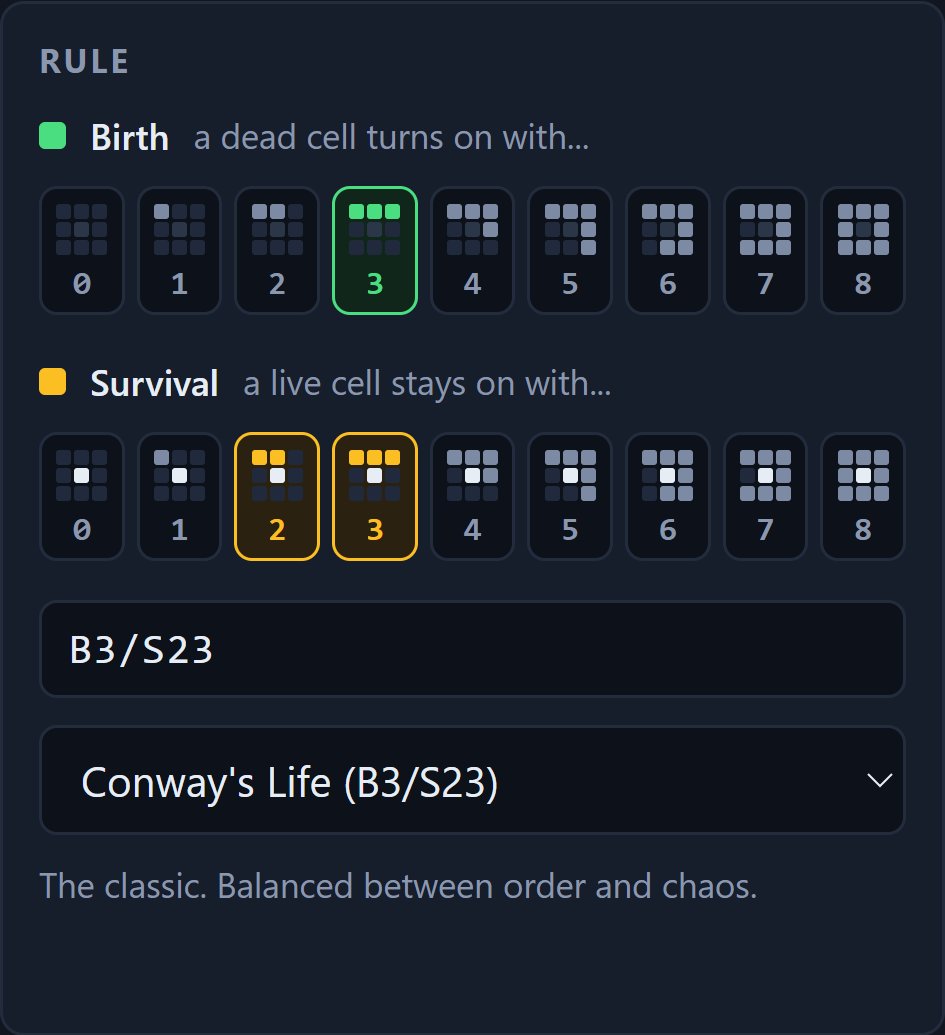
\includegraphics[width=\textwidth]{rule-editor.png}
    \caption{The rule editor. Each toggle draws the neighbourhood situation it controls, so the
    eighteen bits of the rule are visible rather than encoded in a string.}
  \end{subfigure}\hfill
  \begin{subfigure}[t]{0.49\textwidth}
    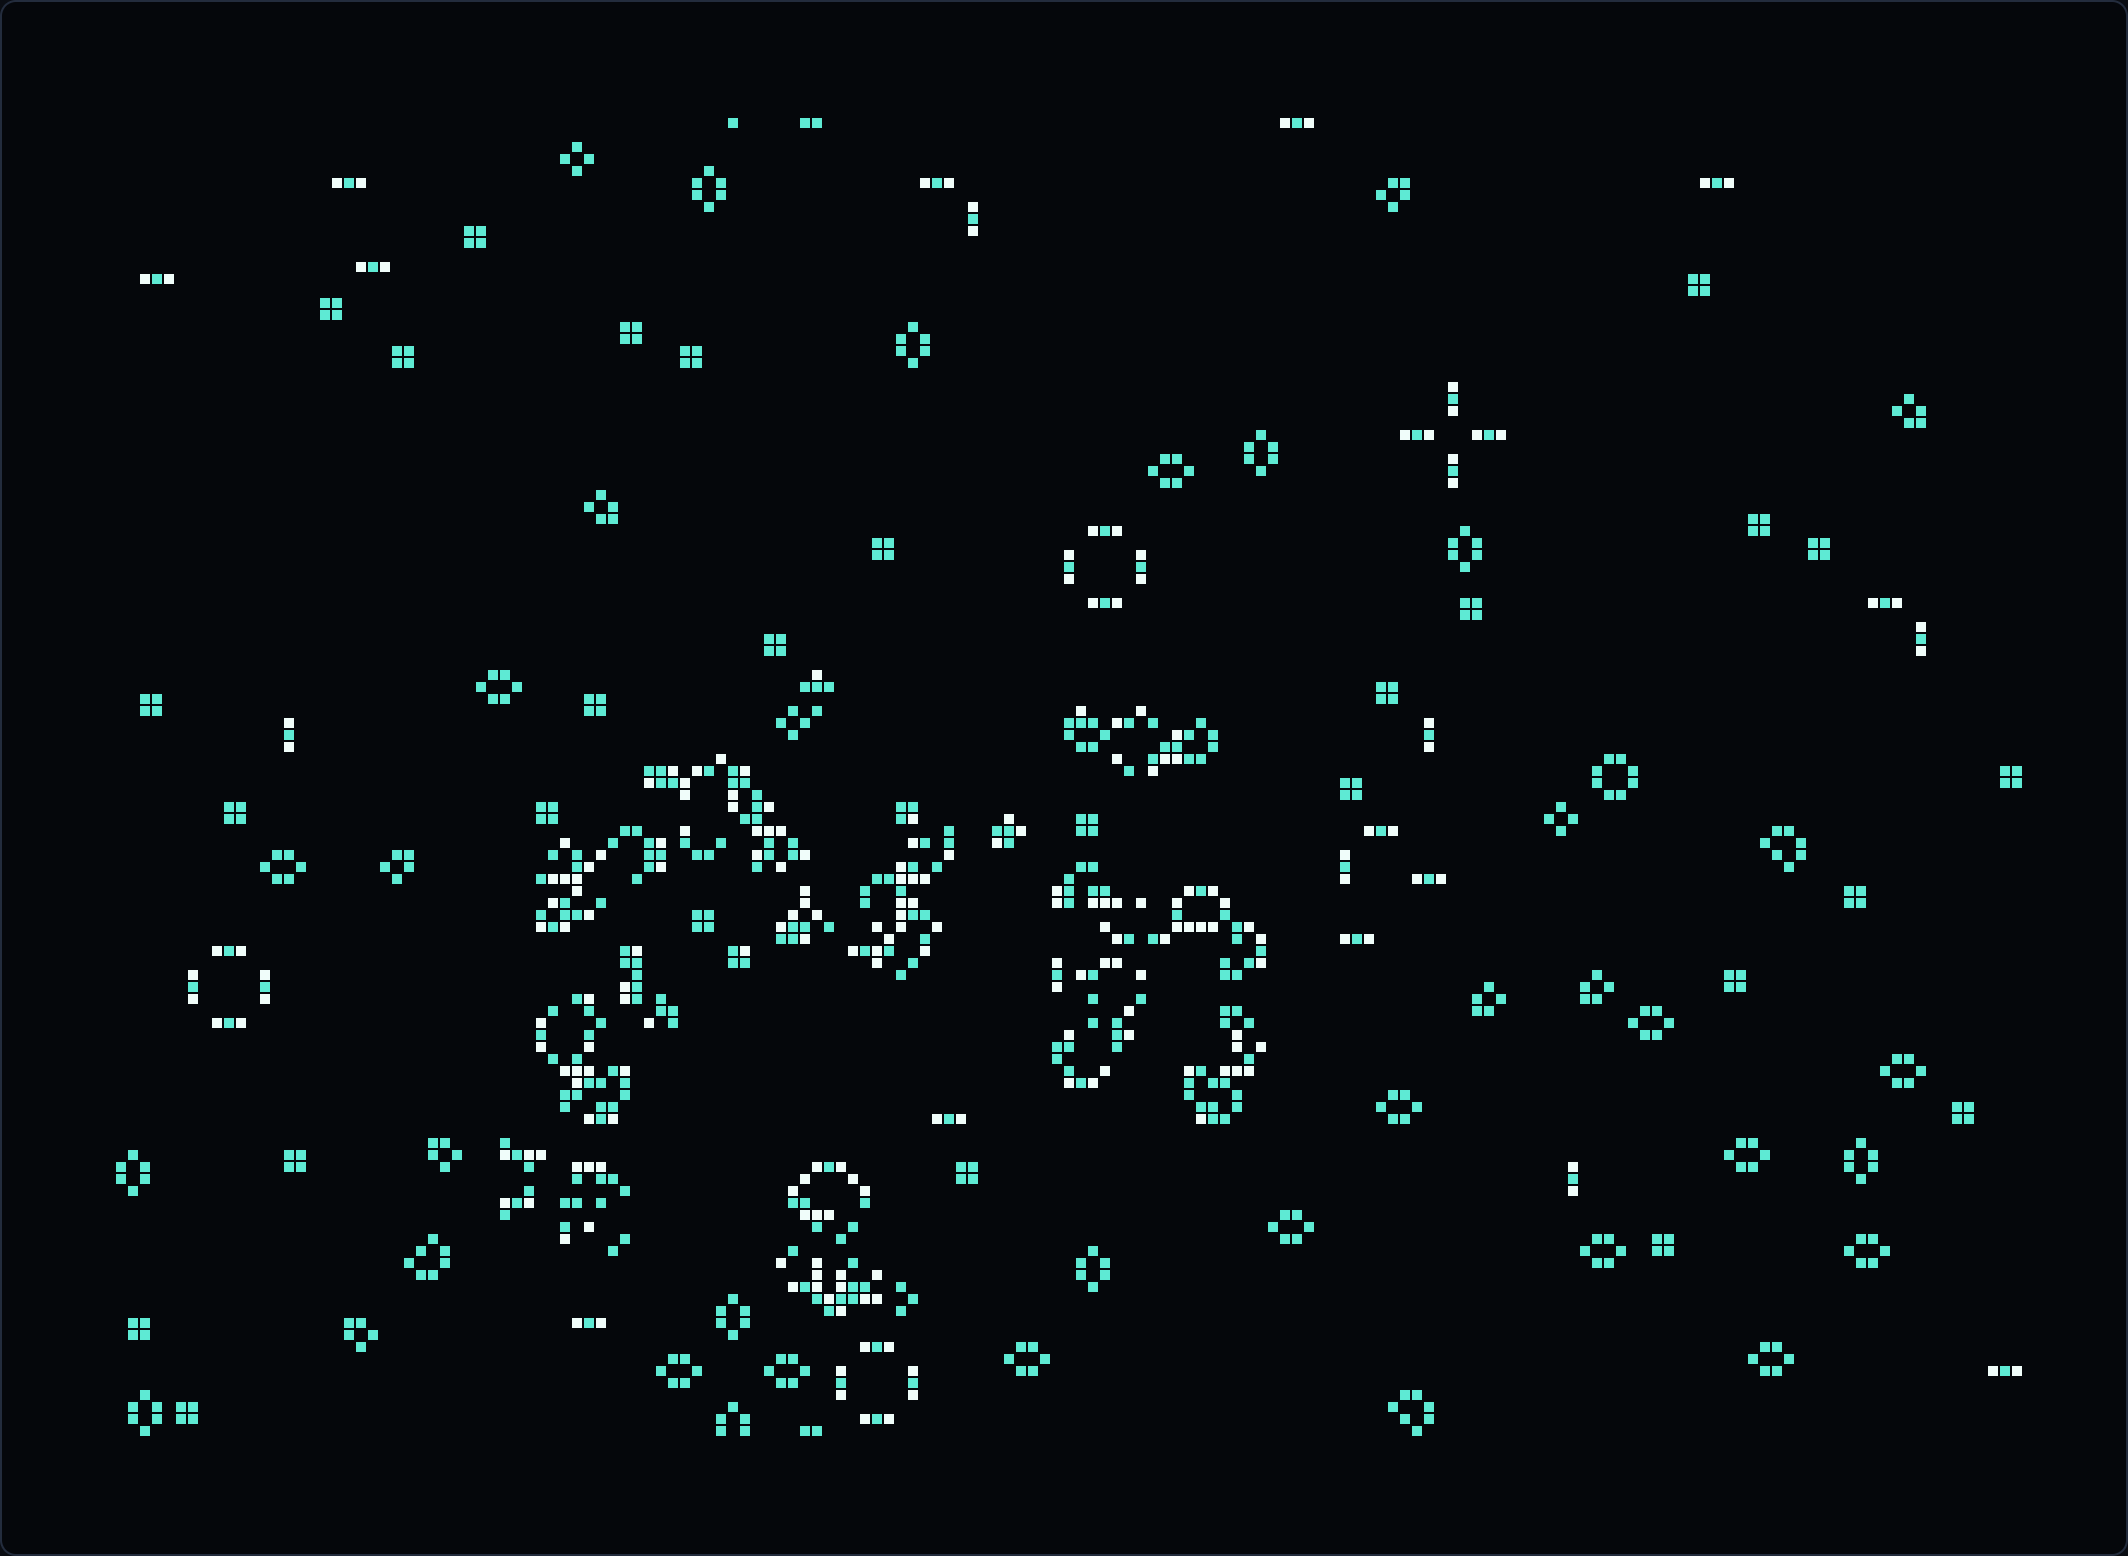
\includegraphics[width=\textwidth]{conway-ash.png}
    \caption{A Conway board after about 1400 generations: sparse islands of a few repeated shapes,
    separated by empty space that nothing in the rule ever mentions.}
  \end{subfigure}
  \caption{The simulator at the end of Task 2.}
\end{figure}

\section{Task 3: what most of the rule space does}

\subsection{Method}

Each rule is run from five random soups on a $64\times64$ torus at densities 5\%, 15\%, 30\%, 50\%
and 75\%, for 800 generations, and four things are measured.

\begin{itemize}
  \item \textbf{Density}, the fraction of live cells, averaged over the last 50 generations.
  \item \textbf{Activity}, the fraction of cells that change state in a generation, averaged over
    the same window. This is the quantity that separates a board frozen into still lifes, which has
    activity zero however full it is, from one that is still boiling.
  \item \textbf{Transient length}, the generation at which the board first repeats a state it has
    already been in, found by hashing every generation.
  \item \textbf{Self-reproduction}, tested directly: a 5-cell seed is run alone and the board is
    checked at every generation for being exactly two or more disjoint translated copies of that
    seed and nothing else. The copies are peeled off greedily, which is exact rather than a
    heuristic, because the topmost-then-leftmost live cell has to be the topmost-then-leftmost cell
    of some copy.
\end{itemize}

Rules are then labelled by cuts through density and activity. The cuts are arbitrary, but they are
stated, reproducible, and applied identically to every rule: extinction below 0.2\% density,
saturating above 50\%, frozen below 0.2\% activity, locally oscillating below 2\%, chaotic above
12\%, and complex in between.

\subsection{Result 1: most of the rule space does one of two boring things}

\begin{table}[h]
\centering
\small
\begin{tabular}{lrrr}
\toprule
class & rules & mean density & mean activity \\
\midrule
extinction & 1 & 0.00\% & 0.00\% \\
frozen & 6 & 5.27\% & 0.04\% \\
locally oscillating & 6 & 20.50\% & 0.69\% \\
complex & 1 & 49.96\% & 8.38\% \\
chaotic & 36 & 39.89\% & 50.21\% \\
saturating & 49 & 64.01\% & 41.57\% \\
self-replicating & 1 & 50.48\% & 49.52\% \\
\bottomrule
\end{tabular}
\caption{100 rules sampled uniformly from the $2^{17}$ rules without B0. 85 of the 100 either fill
the board or boil.}
\end{table}

Eighty-five of a hundred rules either saturate, meaning the board settles above half full, or stay
chaotic, meaning around 40\% of cells are changing state every generation forever. Only 13 do
anything sparse and structured, and those are mostly frozen. Conway's rule is not a typical point in
its own rule space, and it is not close to one.

One rule in the sample, \rulename{B1357/S013578}, passed the self-reproduction test: a 5-cell seed
run alone becomes two disjoint translated copies of itself and nothing else. It is a real
replicator, found by random sampling, but it replicates into a board that is half full and boiling,
so the copies are immediately destroyed by their surroundings.

\paragraph{Half the rule space is spoiled by one bit.} The first sample was drawn uniformly from all
$2^{18}$ rules, and 51 of the 100 contained B0, meaning a dead cell with no live neighbours turns on.
An empty region under such a rule fills instantly, so the entire background of the board flashes on
at the first step and every one of these rules is explosive from the start. That single bit accounts
for half of the rule space and collapses all of it into essentially one behaviour, which is why the
main sample above excludes it: uniform sampling over $2^{18}$ mostly measures B0.

\paragraph{One rule is not one behaviour.} 17 of the 100 rules were labelled differently depending
on which soup they started from. The commonest disagreement is frozen against locally oscillating (4
rules), but three rules went extinct from one initial density and saturated from another, which is as
far apart as two outcomes can be. A single simulation is not evidence about a rule.

\begin{figure}[h]
  \centering
  \begin{subfigure}[t]{0.235\textwidth}
    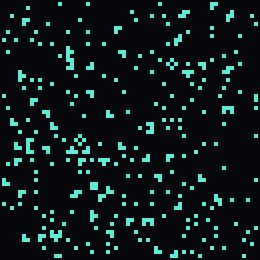
\includegraphics[width=\textwidth]{class-frozen.png}
    \caption*{\small frozen}
  \end{subfigure}\hfill
  \begin{subfigure}[t]{0.235\textwidth}
    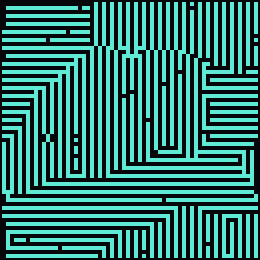
\includegraphics[width=\textwidth]{class-locally-oscillating.png}
    \caption*{\small locally oscillating}
  \end{subfigure}\hfill
  \begin{subfigure}[t]{0.235\textwidth}
    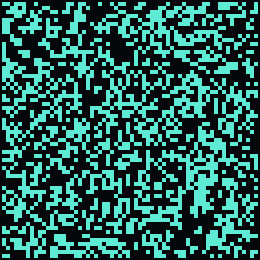
\includegraphics[width=\textwidth]{class-chaotic.png}
    \caption*{\small chaotic}
  \end{subfigure}\hfill
  \begin{subfigure}[t]{0.235\textwidth}
    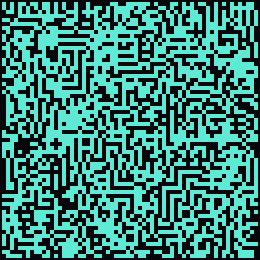
\includegraphics[width=\textwidth]{class-saturating.png}
    \caption*{\small saturating}
  \end{subfigure}
  \caption{One representative of each of the four commonest classes, at generation 800 from a 30\%
  soup on a $64\times64$ torus.}
\end{figure}

\subsection{Result 2: searching instead of sampling}

The sample contains nothing worth a closer look, which the assignment anticipates, so I searched
instead. The search is two stages, and its criterion comes from Task 1 rather than from taste.

\textbf{Stage one} screens 3000 rules without B0 on a single $48\times48$ soup at 30\% density,
keeping those that end between 0.5\% and 15\% full and are still changing at least 0.2\% of their
cells per generation. A rule is abandoned at generation 60 if it is already more than 35\% full,
which is what makes screening thousands of rules affordable: most of the space fills the board within
a few dozen generations and can be rejected there. \textbf{87 of 3000 rules survived, 2.9\%.}

\textbf{Stage two} runs the survivors through the full five-soup measurement and keeps those with the
two properties Conway turned out to have in Task 1: \emph{every} soup settles between 0.2\% and 12\%
full, so the final density is an attractor rather than a reflection of the starting density, and the
board is still changing between 0.1\% and 5\% of its cells per generation. 51 of the 87 passed. The
survivors are ranked by mean transient length, on the grounds that a rule whose soups take hundreds
of generations to resolve is doing more on the way than one that freezes in ten.

The lower end of that density band is calibrated on Conway, and this is worth admitting: my first
version used a floor of 0.5\%, and it rejected Conway's own rule, because Conway's 5\% soup collapses
to 0.44\% full. A filter that rejects the one rule known in advance to be worth finding is a broken
filter, not a strict one.

\textbf{Mobility} is then tested directly rather than inferred. Every pattern that fits in a
$4\times4$ box, one per shape up to rotation and reflection, 7624 of them, is run alone under each
surviving rule until it dies, repeats where it stands, or reappears in the same shape somewhere else.
The test finds the glider under \rulename{B3/S23}, 5 cells and period 4, which is the check that it
works.

\begin{table}[h]
\centering
\small
\begin{tabular}{lrrrr}
\toprule
rule & density & activity & spaceship shapes & score (mean transient) \\
\midrule
\rulename{B368/S0136} & 4.92\% & 0.47\% & 0 & 207 \\
\rulename{B367/S0138} & 5.24\% & 0.61\% & 0 & 176 \\
\rulename{B357/S0248} & 2.15\% & 0.44\% & 0 & 160 \\
\rulename{B37/S01368} & 5.08\% & 0.52\% & 0 & 156 \\
\rulename{B358/S126} & 2.39\% & 0.24\% & \textbf{3} & 117 \\
\midrule
\rulename{B3/S23} (Conway) & 2.41\% & 1.10\% & 2 & 320 \\
\rulename{B36/S23} (HighLife) & 2.79\% & 1.18\% & 2 & 553 \\
\bottomrule
\end{tabular}
\caption{The top of the search, with the two known rules measured the same way for calibration.}
\end{table}

Two things stand out. First, the search works: 51 rules have Conway's macroscopic behaviour, and
several are sparser and more regular than Conway is. Second, none of them beats Conway on the thing
the score actually measures. Conway's transients last 320 generations on this board and HighLife's
553, against 207 for the best rule found. Reproducing the statistics of Conway's steady state turns
out to be much easier than reproducing how long it takes to get there.

The sharpest result is mobility: \textbf{only 3 of the 51 rules have a spaceship at all.} Sparse,
slow and structured is not rare. Sparse, slow, structured \emph{and} able to move information across
the board is rare.

\subsection{A closer look at \rulename{B358/S126}}

I chose the best-scoring rule that also has a spaceship. It is a cleaner version of Conway's
attractor, and a much poorer one in every other respect.

\begin{figure}[h]
  \centering
  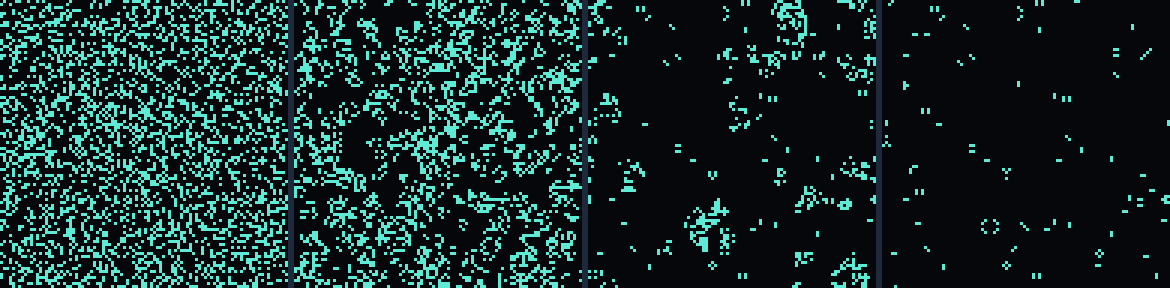
\includegraphics[width=\textwidth]{pick-timeline.png}
  \caption{\rulename{B358/S126} on a $96\times96$ torus at generations 0, 20, 100 and 800 from a 30\%
  soup. The board thins out monotonically and ends as isolated dominoes and diagonal pairs.}
\end{figure}

\begin{table}[h]
\centering
\small
\begin{tabular}{lrrrrrr}
\toprule
& \multicolumn{3}{c}{\rulename{B358/S126}} & \multicolumn{3}{c}{\rulename{B3/S23}} \\
\cmidrule(lr){2-4}\cmidrule(lr){5-7}
initial density & transient & period & final density & \multicolumn{3}{c}{final density} \\
\midrule
5\%  & 19  & 12 & 1.61\% & \multicolumn{3}{c}{0.44\%} \\
15\% & 105 & 12 & 2.56\% & \multicolumn{3}{c}{2.68\%} \\
30\% & 154 & 12 & 1.93\% & \multicolumn{3}{c}{4.21\%} \\
50\% & 151 & 12 & 3.25\% & \multicolumn{3}{c}{4.25\%} \\
75\% & 154 & 12 & 2.61\% & \multicolumn{3}{c}{4.29\%} \\
\bottomrule
\end{tabular}
\caption{Every soup lands in the same narrow band and every one ends in a period-12 cycle. Conway's
figures are from a separate sweep capped at 1200 generations, where many boards have not finished
settling; its fully settled value is about 2.8\%.}
\end{table}

\begin{itemize}
  \item \textbf{The attractor is tighter than Conway's.} Across starting densities from 10\% to 80\%
    the final density stays between 2.1\% and 2.5\%. Conway varies more, and unlike Conway this rule
    does not collapse at 80\%: a very full board thins out to the same 2\% rather than dying of
    overcrowding.
  \item \textbf{Everything has the same period.} All five soups end in a cycle of period 12, and
    every oscillator found in the ash is period 12 as well. Conway's ash is period 1 and 2 with the
    occasional oddity; this rule has one clock and everything runs on it.
  \item \textbf{The vocabulary is poorer.} Conway's ash is dominated by the block, a shape with
    internal structure. This rule leaves mostly 2-cell dominoes and diagonal pairs, 94 of the 105
    isolated structures found. There is nothing here like the loaf or the pond.
  \item \textbf{It does have a spaceship}, 6 cells with period 6, travelling 2 cells straight, so
    speed $c/3$ orthogonally rather than Conway's $c/4$ diagonally. It is in the site's pattern menu
    as \emph{B358 spaceship}, and the rule is in the preset list as \emph{Sparse (searched)}.
\end{itemize}

\begin{center}
\ttfamily\small
\#..\#\\
.\#\#.\\
\#\#..
\end{center}

What this comparison actually taught me is that ``looks like Life'' decomposes into properties that
can be had separately. \rulename{B358/S126} has Life's attractor, more cleanly than Life does. It
does not have Life's long transients, its variety of stable shapes, or anything like the density of
interesting objects. Sparseness is cheap; richness is not.


\section{Task 4, option B: noise and perturbations}

\subsection{What I added, and the choices behind it}

Every cell is flipped independently with probability $p$ after each generation, on or off, regardless
of the rule. The site exposes $p$ on a logarithmic slider from off to $5\times10^{-2}$, and reports
how many of the board's cells that works out to per generation, because $p=10^{-3}$ means nothing
until you know it is 18 cells on a $160\times110$ board.

Three implementation choices are worth stating.

\paragraph{Symmetric flips, not injections.} A cell that is on can be turned off and a cell that is
off can be turned on, with the same probability. This is the reading of the assignment's ``randomly
turn cells on or off'', and it is the choice with the fewest parameters, but it is not neutral: a
Conway board is about 97\% dead, so in practice almost every flip is a spontaneous birth. A model
with separate on and off rates would be a different experiment, and Section~6 lists it as a
limitation.

\paragraph{Sampling the gaps, not the cells.} Drawing one random number per cell would cost 104{,}000
random numbers per generation on the largest board, which is more work than the rule itself. Instead
\texttt{applyNoise} draws the gap to the next flipped cell straight from the geometric distribution
that governs it, so the cost is proportional to the number of flips rather than to the size of the
board. It is exact, not an approximation, and it is asserted in the tests.

\paragraph{Noise turns the cycle detector off.} The site normally announces when a board freezes or
falls into a cycle, by hashing generations and looking for a repeat. Under noise a repeat would not
mean a cycle, because the rule is no longer the only thing changing the board, so the detector is
disabled and the board reports itself as perturbed instead. For the same reason an empty board no
longer pauses the simulation when noise is on: with noise, extinction is temporary.

Cells the noise flipped on are painted amber rather than the usual white-for-newly-born, which turned
out to matter more than expected. Watching a single amber cell appear next to a block and then
watching the block turn into something else is the whole of Section~5.4 in one image.

\begin{figure}[t]
  \centering
  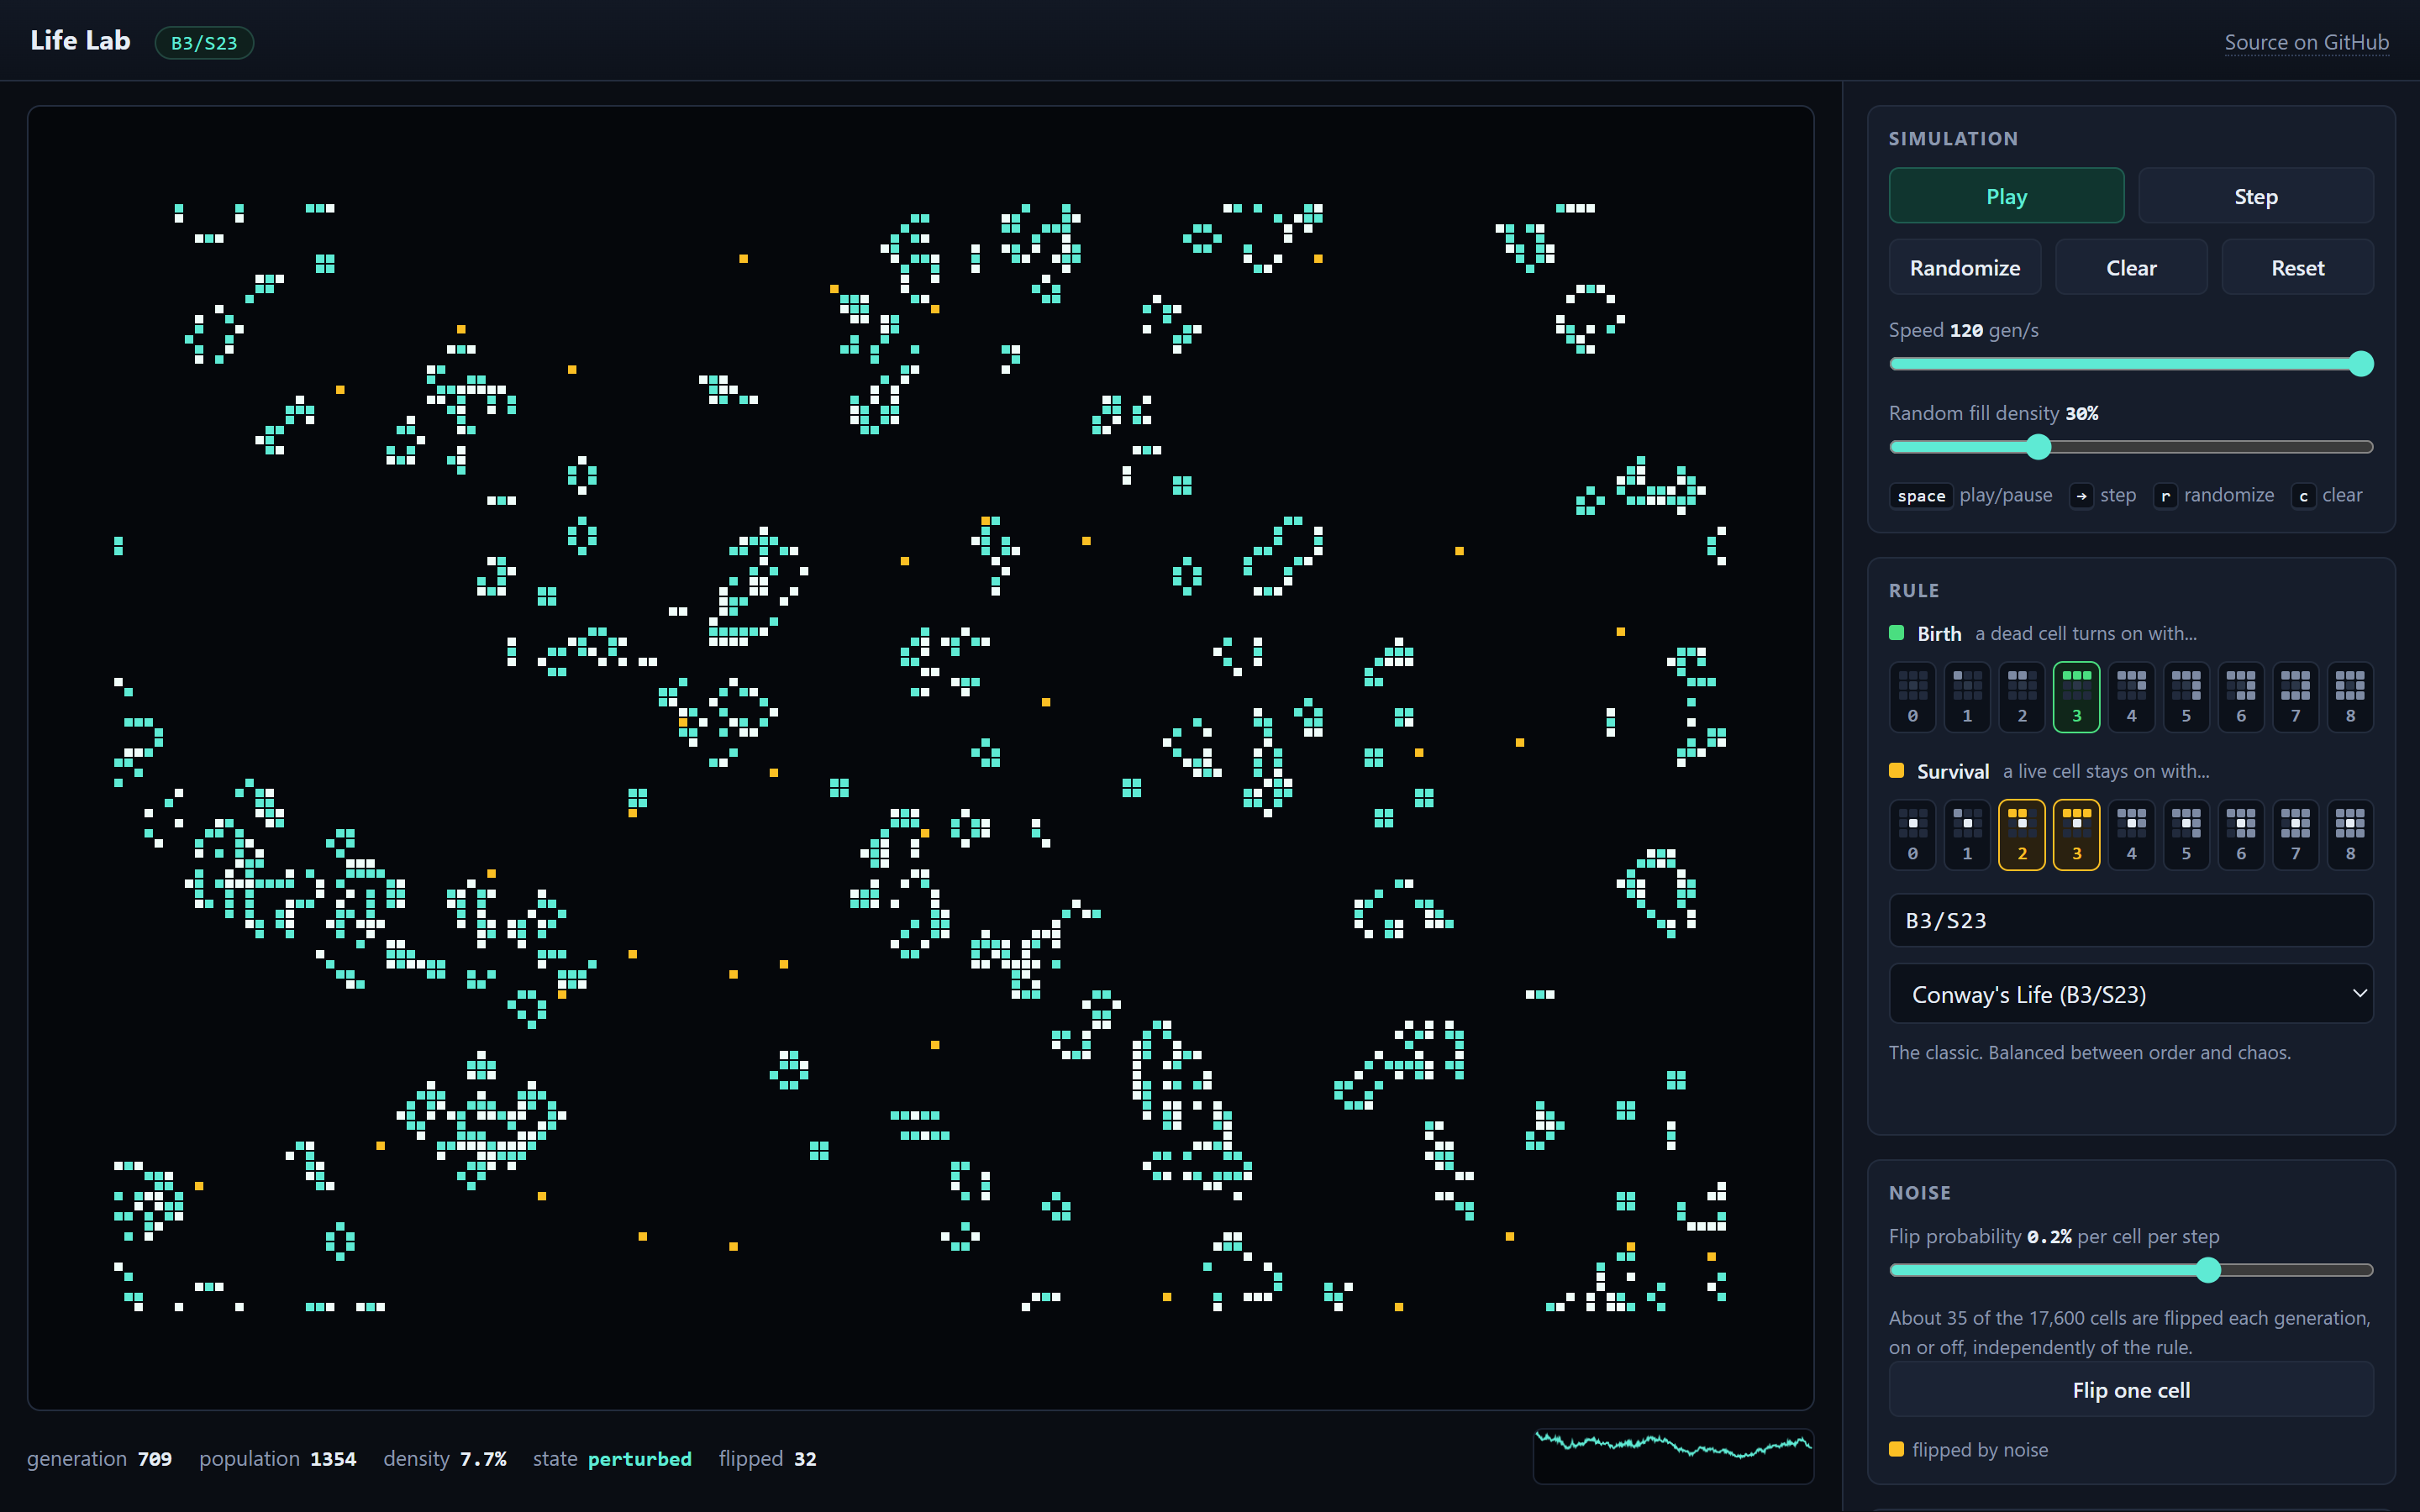
\includegraphics[width=0.86\textwidth]{noise-ui.png}
  \caption{Conway's Life at $p=2\times10^{-3}$, generation 709. Amber cells are the 32 the noise
  flipped this step, white cells were born by the rule, teal cells survived. The board is 7.7\% full
  against the 2.8\% it settles to with no noise, and the sparkline at the bottom right is flat rather
  than decaying: the board never settles.}
\end{figure}

\subsection{Method}

Four experiments, all on a torus, all with a seeded generator.

\begin{enumerate}[leftmargin=1.4em]
  \item \textbf{Steady state against noise rate.} A $96\times96$ soup at 30\% density is run for 700
    generations of burn-in and 700 of measurement, and the density and the activity are averaged
    over the second half. Flips injected by the noise are not counted as activity, so activity
    measures what the rule is doing rather than what was put in.
  \item \textbf{Structure lifetimes.} One structure is placed alone on a $32\times32$ torus with
    noise. A noise-free copy runs in lockstep and defines what the structure should look like at
    every generation, which handles oscillators and spaceships without special cases: the structure
    is intact while the noisy board agrees with the reference everywhere within two cells of the
    reference structure. Damage that the rule repairs within four generations does not count, so
    what is timed is damage that sticks.
  \item \textbf{Which single flips are fatal.} The same question without the statistics: every cell
    within two of a structure is flipped once, on its own, with no other noise, and the board is run
    for 96 generations to see whether the structure comes back.
  \item \textbf{Damage spreading.} Two boards that differ in exactly one cell are driven by
    \emph{identical} noise for 400 generations after a 600-generation burn-in. Sharing the noise is
    the point: any difference left at the end is caused by the one flip that separates the boards,
    not by the perturbations themselves, so the final Hamming distance says whether the noisy steady
    state absorbs a disturbance or amplifies it.
\end{enumerate}

\subsection{Result 1: Life is fed by noise; the searched rule is eroded by it}

\begin{figure}[h]
\centering
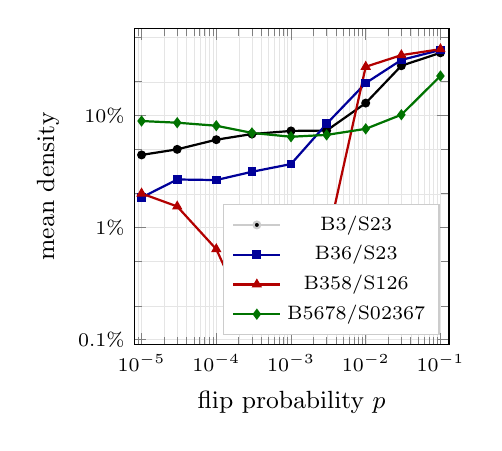
\begin{tikzpicture}
\begin{loglogaxis}[
  width=0.46\textwidth, height=5.6cm,
  xlabel={flip probability $p$}, ylabel={mean density},
  ymin=0.09, ymax=60, xmin=8e-6, xmax=1.3e-1,
  ytick={0.1,1,10}, yticklabels={0.1\%,1\%,10\%}, minor ytick={0.2,0.5,2,5,20,50},
  legend pos=south east, legend style={font=\scriptsize,draw=gray!40,fill=white},
  grid=both, grid style={line width=.1pt,draw=gray!20},
  tick label style={font=\scriptsize}, label style={font=\small},
]
\addplot[thick,mark=*,mark size=1.2] coordinates {(1e-5,4.44)(3e-5,4.98)(1e-4,6.07)(3e-4,6.82)(1e-3,7.27)(3e-3,7.33)(1e-2,12.89)(3e-2,27.75)(1e-1,36.19)};
\addlegendentry{B3/S23}
\addplot[thick,mark=square*,mark size=1.2,color=blue!60!black] coordinates {(1e-5,1.85)(3e-5,2.68)(1e-4,2.65)(3e-4,3.14)(1e-3,3.68)(3e-3,8.42)(1e-2,19.44)(3e-2,31.26)(1e-1,38.40)};
\addlegendentry{B36/S23}
\addplot[thick,mark=triangle*,mark size=1.4,color=red!70!black] coordinates {(1e-5,2.01)(3e-5,1.54)(1e-4,0.64)(3e-4,0.13)(1e-3,0.19)(3e-3,0.74)(1e-2,27.19)(3e-2,34.50)(1e-1,39.03)};
\addlegendentry{B358/S126}
\addplot[thick,mark=diamond*,mark size=1.4,color=green!45!black] coordinates {(1e-5,8.91)(3e-5,8.61)(1e-4,8.09)(3e-4,6.98)(1e-3,6.45)(3e-3,6.70)(1e-2,7.59)(3e-2,10.14)(1e-1,22.49)};
\addlegendentry{B5678/S02367}
\end{loglogaxis}
\end{tikzpicture}
\hfill
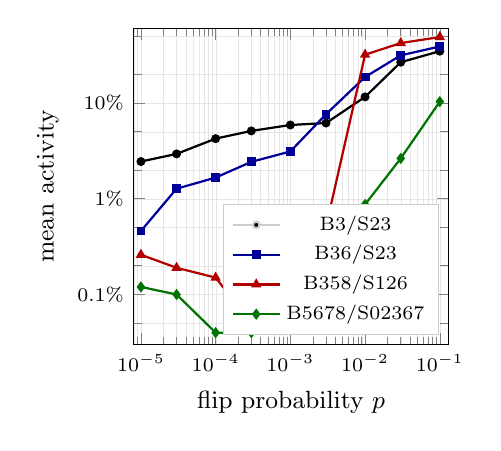
\begin{tikzpicture}
\begin{loglogaxis}[
  width=0.46\textwidth, height=5.6cm,
  xlabel={flip probability $p$}, ylabel={mean activity},
  ymin=0.03, ymax=60, xmin=8e-6, xmax=1.3e-1,
  ytick={0.1,1,10}, yticklabels={0.1\%,1\%,10\%}, minor ytick={0.05,0.2,0.5,2,5,20,50},
  legend pos=south east, legend style={font=\scriptsize,draw=gray!40,fill=white},
  grid=both, grid style={line width=.1pt,draw=gray!20},
  tick label style={font=\scriptsize}, label style={font=\small},
]
\addplot[thick,mark=*,mark size=1.2] coordinates {(1e-5,2.44)(3e-5,2.93)(1e-4,4.23)(3e-4,5.09)(1e-3,5.87)(3e-3,6.15)(1e-2,11.53)(3e-2,26.51)(1e-1,34.57)};
\addlegendentry{B3/S23}
\addplot[thick,mark=square*,mark size=1.2,color=blue!60!black] coordinates {(1e-5,0.46)(3e-5,1.27)(1e-4,1.66)(3e-4,2.42)(1e-3,3.11)(3e-3,7.60)(1e-2,18.59)(3e-2,31.28)(1e-1,38.70)};
\addlegendentry{B36/S23}
\addplot[thick,mark=triangle*,mark size=1.4,color=red!70!black] coordinates {(1e-5,0.26)(3e-5,0.19)(1e-4,0.15)(3e-4,0.05)(1e-3,0.12)(3e-3,0.51)(1e-2,31.79)(3e-2,42.00)(1e-1,48.55)};
\addlegendentry{B358/S126}
\addplot[thick,mark=diamond*,mark size=1.4,color=green!45!black] coordinates {(1e-5,0.12)(3e-5,0.10)(1e-4,0.04)(3e-4,0.04)(1e-3,0.09)(3e-3,0.26)(1e-2,0.87)(3e-2,2.63)(1e-1,10.28)};
\addlegendentry{B5678/S02367}
\end{loglogaxis}
\end{tikzpicture}
\caption{Steady state against noise rate, $96\times96$ torus, averaged over the last 700 of 1400
generations and three seeds. With no noise the four rules sit at 3.40\%, 2.65\%, 2.22\% and 9.02\%
density and 1.31\%, 0.61\%, 0.23\% and 0.13\% activity.}
\end{figure}

\paragraph{There is no lower threshold: Life's frozen state is only metastable.} One flip every
eleven generations, $p=10^{-5}$ on this board, is enough to take Conway from 3.40\% density and
1.31\% activity to 4.44\% and 2.44\%. There is no rate small enough to be ignored, because the
noise-free end state is not stable, only motionless: a board of still lifes stays put because nothing
disturbs it, and a single disturbed cell restarts local activity that then never stops. Whatever
threshold exists is at the top of the range, not the bottom.

\paragraph{Two rules that look alike respond in opposite directions.} \rulename{B358/S126}, the rule
from Task 3 that reproduces Conway's attractor more tightly than Conway does, is \emph{destroyed} by
the same noise that feeds Conway: its density falls from 2.22\% to 0.13\% by $p=3\times10^{-4}$,
seventeen times emptier, before the noise eventually overwhelms everything at $p=10^{-2}$. Conway's
ash gets denser under noise and this rule's ash gets thinner. Its stable objects are mostly 2-cell
dominoes, which are the smallest thing that can persist at all, and a domino has no margin: any
neighbour it acquires puts its cells outside the survival counts. Conway's block is bigger and can
absorb more before it stops being a block. Two rules with the same steady state can have completely
different relationships with perturbation, and nothing in the Task 3 measurements would have
predicted which.

\paragraph{Chaotic and saturating rules do not notice.} \rulename{B25/S2468} sits at 39.2\% density
and 40.6\% activity at every noise rate from $0$ to $10^{-2}$, changing in the third significant
figure. Noise is invisible against a system that is already generating disorder faster than the noise
supplies it. Sensitivity to perturbation is a property of \emph{ordered} states.

\subsection{Result 2: Life almost never repairs damage}

The clearest measurement in the project takes no statistics at all. For each structure, every cell
within two of it was flipped once, on its own, and the board run for 96 generations to see whether
the structure came back.

\begin{table}[h]
\centering
\small
\begin{tabular}{lrrrrrr}
\toprule
structure & cells & neighbourhood & fatal flips & fatal & predicted lifetime & measured \\
\midrule
blinker & 3 & 35 & 25 & 71\% & 40 & 47 \\
tub & 4 & 45 & 25 & 56\% & 40 & 45 \\
block & 4 & 36 & 28 & 78\% & 36 & 44 \\
boat & 5 & 46 & 33 & 72\% & 30 & 39 \\
glider & 5 & 46 & 33 & 72\% & 30 & 31 \\
beehive & 6 & 52 & 38 & 73\% & 26 & 32 \\
toad & 6 & 46 & 34 & 74\% & 29 & 30 \\
loaf & 7 & 58 & 43 & 74\% & 23 & 28 \\
pond & 8 & 60 & 52 & 87\% & 19 & 23 \\
beacon & 8 & 56 & 50 & 89\% & 20 & 24 \\
lightweight spaceship & 9 & 70 & 52 & 74\% & 19 & 25 \\
\bottomrule
\end{tabular}
\caption{Single-flip census under \rulename{B3/S23}. ``Predicted lifetime'' is $1/(p\,F)$ at
$p=10^{-3}$, where $F$ is the number of fatal flips; ``measured'' is the mean over 40 noisy runs.
Lifetimes are in generations.}
\end{table}

\begin{itemize}
  \item \textbf{Between 56\% and 89\% of single flips near a structure destroy it permanently.} Life
    has no repair mechanism. A structure is stable in the sense that it does not change on its own,
    not in the sense that it returns after being pushed.
  \item \textbf{The one-flip census predicts the noisy lifetimes.} Taking $1/(pF)$ as the expected
    time until a fatal flip lands reproduces the measured mean lifetime to within 25\% for every
    structure, and to within a few percent for several. The mechanism is simply the first fatal flip.
    The measured lifetimes are slightly longer than predicted throughout, which is what should happen
    given that a flip is only counted as damage once it has persisted four generations.
  \item \textbf{Robustness is almost entirely size.} Ranking the structures by lifetime gives
    blinker, tub, block, boat, glider, beehive, toad, loaf, pond, beacon, lightweight spaceship,
    which is very nearly the ranking by the size of their neighbourhood, smallest first. A big
    structure presents more surface to be hit. The pond, 8 cells, survives half as long as the
    blinker, 3 cells.
  \item \textbf{Big structures are much worse off than this table suggests.} At
    $p=3\times10^{-4}$ the pulsar lasts 15 generations, the Gosper glider gun 13, and the HighLife
    replicator 26. The gun is 36 cells and its neighbourhood is nearly 300; that a machine capable
    of unbounded growth is destroyed in 13 generations by three flips per generation somewhere on a
    $96\times96$ board is the sharpest statement of the fragility here.
  \item \textbf{Moving does not help.} A glider is no more robust than a still life of the same size,
    and the lightweight spaceship is among the least robust things measured. A spaceship sweeps new
    territory, so it meets fresh noise rather than escaping it.
\end{itemize}

Two smaller observations. Under \rulename{B25/S2468} and \rulename{B2456/S156} the same block and
blinker last 7 to 11 generations rather than 44 to 47: in a chaotic or saturating rule, the structure
is destroyed by the board's own products before the noise gets to it. And Conway and HighLife give
\emph{identical} lifetimes, 44 and 47, because neither the structures nor the sparse debris around
them ever presents a cell with six live neighbours, so at low density the two rules are the same rule.

\subsection{Result 3: where the behaviour changes character}

Three independent measurements were used to look for a threshold, and they agree.

\begin{figure}[h]
\centering
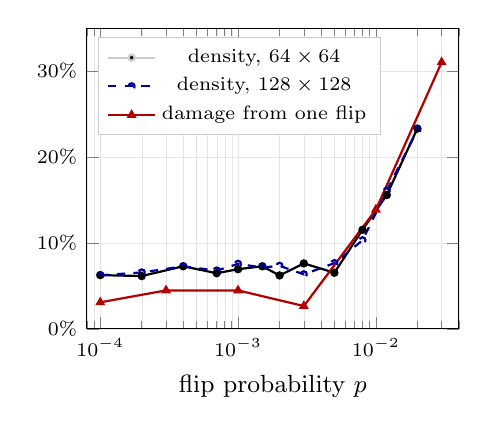
\begin{tikzpicture}
\begin{semilogxaxis}[
  width=0.52\textwidth, height=5.4cm,
  xlabel={flip probability $p$}, ylabel={},
  ymin=0, ymax=35, xmin=8e-5, xmax=4e-2,
  legend pos=north west, legend style={font=\scriptsize,draw=gray!40,fill=white},
  grid=both, grid style={line width=.1pt,draw=gray!20},
  tick label style={font=\scriptsize}, label style={font=\small},
  yticklabel={\pgfmathprintnumber{\tick}\%},
]
\addplot[thick,mark=*,mark size=1.1] coordinates {(1e-4,6.26)(2e-4,6.15)(4e-4,7.29)(7e-4,6.48)(1e-3,6.95)(1.5e-3,7.29)(2e-3,6.22)(3e-3,7.62)(5e-3,6.54)(8e-3,11.54)(1.2e-2,15.58)(2e-2,23.32)};
\addlegendentry{density, $64\times64$}
\addplot[thick,dashed,mark=o,mark size=1.1,color=blue!60!black] coordinates {(1e-4,6.24)(2e-4,6.57)(4e-4,7.28)(7e-4,6.79)(1e-3,7.57)(1.5e-3,7.14)(2e-3,7.34)(3e-3,6.35)(5e-3,7.65)(8e-3,10.31)(1.2e-2,16.08)(2e-2,23.16)};
\addlegendentry{density, $128\times128$}
\addplot[thick,mark=triangle*,mark size=1.3,color=red!70!black] coordinates {(1e-4,3.09)(3e-4,4.48)(1e-3,4.48)(3e-3,2.66)(1e-2,13.88)(3e-2,31.03)};
\addlegendentry{damage from one flip}
\end{semilogxaxis}
\end{tikzpicture}
\hfill
\begin{minipage}[b]{0.44\textwidth}
\small
\begin{tabular}{lrr}
\toprule
$p$ & healed & mean damage \\
\midrule
0 & 15/20 & 1.74\% \\
$3\times10^{-5}$ & 17/20 & 1.27\% \\
$10^{-4}$ & 14/20 & 3.09\% \\
$3\times10^{-4}$ & 13/20 & 4.48\% \\
$10^{-3}$ & 14/20 & 4.48\% \\
$3\times10^{-3}$ & 16/20 & 2.66\% \\
$10^{-2}$ & \textbf{8/20} & \textbf{13.88\%} \\
$3\times10^{-2}$ & \textbf{4/20} & \textbf{31.03\%} \\
\bottomrule
\end{tabular}
\captionof{table}{Two boards differing in one cell, driven by identical noise.}
\end{minipage}
\caption{Conway across the transition. Density plateaus near 7\% up to $p\approx5\times10^{-3}$ and
then climbs; the damage from a single flip is contained below that and spreads above it. The two
board sizes agree throughout, so the change is not a finite-size artefact.}
\end{figure}

\begin{enumerate}[leftmargin=1.4em]
  \item \textbf{Density plateaus and then climbs.} From $p=10^{-4}$ to $p=5\times10^{-3}$, a factor
    of fifty, Conway's steady-state density stays between 6.2\% and 7.6\%, which is within the
    scatter of the measurement. Above that it climbs steadily: 11.5\% at $8\times10^{-3}$, 15.6\% at
    $1.2\times10^{-2}$, 23.3\% at $2\times10^{-2}$.
  \item \textbf{Activity does the same thing.} It tracks the density closely, which is itself
    informative: above the knee the board is not a denser ash, it is a boiling state where density
    and activity are the same number.
  \item \textbf{Damage from a single flip stops being contained.} Below $3\times10^{-3}$, 13 to 17
    of every 20 single-cell perturbations heal completely even though the noise keeps running, and
    the mean surviving damage is 1\% to 4\% of the board. At $10^{-2}$ only 8 of 20 heal and the
    damage is 14\% of the board; at $3\times10^{-2}$, 4 of 20 and 31\%.
\end{enumerate}

So there is a threshold, at $p\approx6\times10^{-3}$, but it is a crossover rather than a sharp
transition: the curves bend over a factor of two or three in $p$ rather than jumping, and doubling
the board size does not sharpen them, which is what would be expected of a genuine phase transition.
Calling it a phase transition would be overclaiming from this data.

There is a simple reading of where the number comes from. The mean time until a fatal flip lands in a
given structure's neighbourhood is about $1/(pF)$, roughly $1/30p$ generations. At
$p=6\times10^{-3}$ that is about 6 generations, which is the same order as the time a small
disturbance takes to settle down into new stable debris, a few tens of generations. Below the
threshold, structures are destroyed more slowly than the board can rebuild them, and an ash exists in
the steady state. Above it, they are destroyed faster than they can form, and there is no ash to
disturb. This is consistent with the numbers rather than derived from them, but it does predict the
right order of magnitude, and it explains why the threshold sits where it does rather than anywhere
else.

\begin{figure}[h]
  \centering
  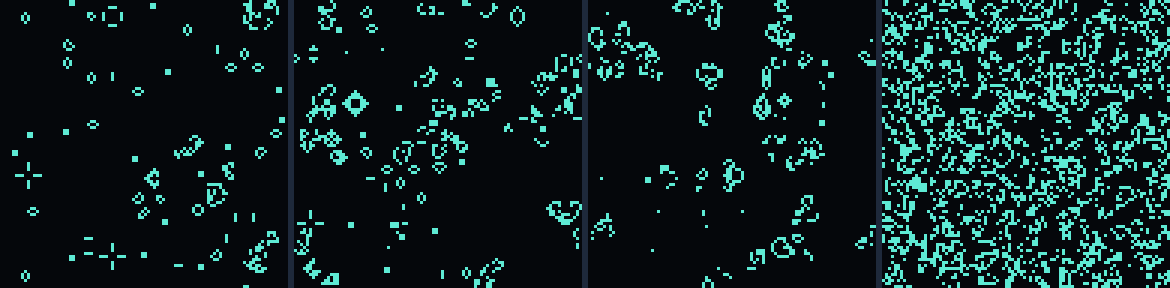
\includegraphics[width=\textwidth]{noise-conway-strip.png}
  \caption{Conway's Life after 1200 generations at $p=0$, $3\times10^{-4}$, $3\times10^{-3}$ and
  $3\times10^{-2}$. The first three straddle a factor of ten in noise and look much the same, which
  is the plateau; the fourth is on the other side of the threshold and has no structures left in it
  at all.}
\end{figure}

\subsection{Result 4: one flip on a settled board}

Finally, the noise-free case, which is what the \emph{Flip one cell} button on the site does. Sixty
Conway soups were run until the board entered a cycle, one cell was flipped, and the flipped board
was compared with the untouched one for 400 generations.

\textbf{52 of 60 healed completely}, meaning the two boards became identical again. In the 8 that did
not, the difference peaked at 81 cells on average. Settled Conway ash is therefore mostly, but not
reliably, insensitive to a single perturbation, and the failures are not small: when a flip does
survive, it typically restarts a region rather than leaving a small scar. That combination, usually
nothing and occasionally a lot, is the same shape as the fatal-flip census: most of the board is
empty, a flip in empty space dies immediately, and a flip that lands near a structure destroys it
about three quarters of the time.


\section{How I used AI}

I used Claude Code, Anthropic's command-line agent, throughout the project, and it wrote most of the
code. The division of labour was roughly this.

\begin{itemize}
  \item \textbf{Implementation.} The engine, the React interface, the rule editor, the noise
    controls, and all of the experiment scripts were written by the agent from prompts describing
    what I wanted. I reviewed the code, asked for changes when it was more complicated than the
    problem needed, and read through anything I did not understand until I did.
  \item \textbf{Experiment design.} This was the most useful part and the most collaborative. I
    would say what I wanted to know, for example ``which patterns are robust under noise'', and we
    would go back and forth on what would actually measure that. Several of the definitions in this
    report came out of those exchanges: the idea of running a noise-free reference board in lockstep
    to define what a structure ``should'' look like, and the idea of driving two boards with
    identical noise so that any surviving difference is attributable to the single flip that
    separates them.
  \item \textbf{Debugging.} Two of the more useful moments were failures. The pattern catalogue is
    tested by asserting the behaviour each description claims, and that caught a ``replicator'' that
    simply died after 5 generations. Rather than guess again, we enumerated every pattern in a
    $5\times5$ box with 5, 6 or 7 cells, about 470{,}000 of them, and ran each for 24 generations
    looking for one that becomes two translated copies of itself. There were none, which proved the
    replicator had to be larger and ruled out a whole class of guesses at once. Separately, a bug in
    a test helper made the pulsar and the Gosper gun look broken when both were correct, which was a
    good reminder that the measuring instrument is part of what needs checking.
  \item \textbf{Learning.} I used it to explain things I had not met before: outer-totalistic rule
    notation, why damage spreading is the standard way to ask whether a perturbation is amplified,
    and what a finite-size check is for.
  \item \textbf{Making this Writeup.} I used it to summarize the results of this investigation into
    a well-formatted .tex file and generate the graphics and figures.
\end{itemize}

However, most of the experimentation was driven by myself with Claude as a secondary guide. I
personally observed the simulations and classified the rulesets myself.

\section{Limitations}

\begin{itemize}
  \item \textbf{Board size and run length.} Everything here runs on boards between $32\times32$ and
    $128\times128$ for at most a few thousand generations. Conway soups on a $96\times96$ torus
    routinely take 1200 to 1800 generations to settle, so the boards are only about one order of
    magnitude larger than the structures they contain. Some of what I call a steady state may be a
    finite-size effect.
  \item \textbf{Classification by thresholds.} The rule classes in Section~4 are cuts through two
    measured numbers. They are reproducible and stated explicitly, but the boundaries are mine, and
    a rule sitting near one of them could be labelled either way. The measurement that a rule can
    change class depending on its initial density makes this concrete.
  \item \textbf{The search is not a proof.} Screening 3000 rules found candidates that satisfy two
    properties Conway has. That is not the same as finding a rule that is interesting in the way
    Conway is interesting, which involves things I did not measure at all, such as whether the rule
    supports guns, computation, or stable long-range signalling.
  \item \textbf{Noise model.} I used one noise model: each cell flips independently with the same
    probability at every step. Noise that only turns cells on, or only off, or that is correlated in
    space, would probably behave differently, and the asymmetry matters because a sparse board has
    far more dead cells than live ones, so symmetric flipping is mostly an injection of new life.
  \item \textbf{Statistics.} Most points here are 3 to 40 trials. That is enough to see effects of a
    factor of two but not enough to pin down an exponent, and the non-monotonic wobble in the
    finite-size table is sampling noise rather than structure.
\end{itemize}

\section{General thoughts}

The result that surprised me most was from Task 1 and I keep coming back to it: a board that starts
10\% full and a board that starts 70\% full both end up at about 3\% full. Nothing in
\rulename{B3/S23} mentions densities, or regions, or boundaries. The rule only ever counts to eight.
The fact that a fixed point exists at all, and that it is the same fixed point from almost any
starting condition, is the clearest thing in the project, and it is the reason the phrase
``self-organisation'' stopped being an abstraction for me.

The second thing that stuck was how rare interesting rules are. Roughly 85\% of a random sample
either fills the board or boils, half the rule space is spoiled by a single bit, and after screening
3000 rules only about 2\% were even worth measuring properly. Conway's rule is not a typical point in
its own rule space. Whether that is a fact about cellular automata or a fact about what humans find
interesting is a question I would like to think about more.

The third is from Task 4: Life does not repair itself. Almost every flip that lands within
two cells of a structure destroys that structure, and what looks like stability is really the
absence of anything trying to knock it over. That is a real difference from biological systems,
which repair damage actively, and it makes me want to know whether there are rules in this space that
do repair, and what a rule would have to look like for repair to be possible at all.

What I would like to learn more about, in order: larger neighbourhoods and continuous states, since
Lenia and SmoothLife seem to get much more organism-like behaviour out of the same idea; how to
search rule spaces properly rather than with the hand-built filter I used here; and whether anything
in this space can be made to undergo selection rather than just reproduction, because the HighLife
replicator copies itself perfectly and that turns out to be exactly the wrong property for evolution.

\section{Reproducing this}

\begin{verbatim}
npm install
npm test                        # 31 engine and pattern tests
npm run dev                     # the site, at http://localhost:3000
node scripts/survey.mjs         # Tasks 1 and 2  -> docs/survey-output.md
node scripts/rule-survey.mjs    # Task 3         -> docs/rule-survey-output.md
node scripts/noise-survey.mjs   # Task 4         -> docs/noise-output.md
\end{verbatim}

\noindent
On the site, the two headline observations can be reproduced by hand. For Task 1, set the density
slider anywhere between 10\% and 70\%, press Randomize, then Play at 120 generations per second and
watch the population sparkline flatten at roughly the same level whatever density you started from.
For Task 4, do the same and then raise the noise slider one notch at a time: at
$p=10^{-4}$ the ash keeps being disturbed and rebuilt, and at $p=10^{-2}$ there is no ash left to
disturb.

\end{document}

